% Restructured book: solution for problem 1.
\chapter{Solution for Problem 1: Automatic Layout Design}

Chapter 1 identified the need for an initial furniture layout that is both geometrically usable and easy to revise. This chapter presents the pipeline that turns a natural-language brief, explicit room geometry, and available furniture into that editable layout. The result is structured room-and-object data rather than a static image, so it can be validated against spatial constraints and reused by the 2D editor, 3D preview, and layout-conditioned image workflow.

\section{Overall Processing Flow}\label{sec:problem1-processing-flow}

The automatic layout-generation pipeline starts from three main inputs: the user's design brief, the room geometry, and the furniture inventory. The design brief describes the intended room type, activities, style, required objects, and user preferences. The room geometry provides the boundary polygon, doors, windows, and room height. The furniture inventory provides object categories, dimensions, style metadata, material metadata, and optional 3D assets.

The example brief is: ``compact guest bedroom with a bed, wardrobe, desk, and a small vanity near the window''. The room is a 4.0 m by 3.2 m rectangle with one door on the south wall and one window on the north wall. The semantic modules infer that the bed and wardrobe are required, the desk is strongly preferred, and the vanity is preferred if space allows. The room model converts the door and window into clearance and daylight zones. The object program turns these requirements into anchors and support objects, and the solver searches for placements that keep the door clear, avoid overlap, and preserve circulation.

\begin{figure}[!htbp]
\centering
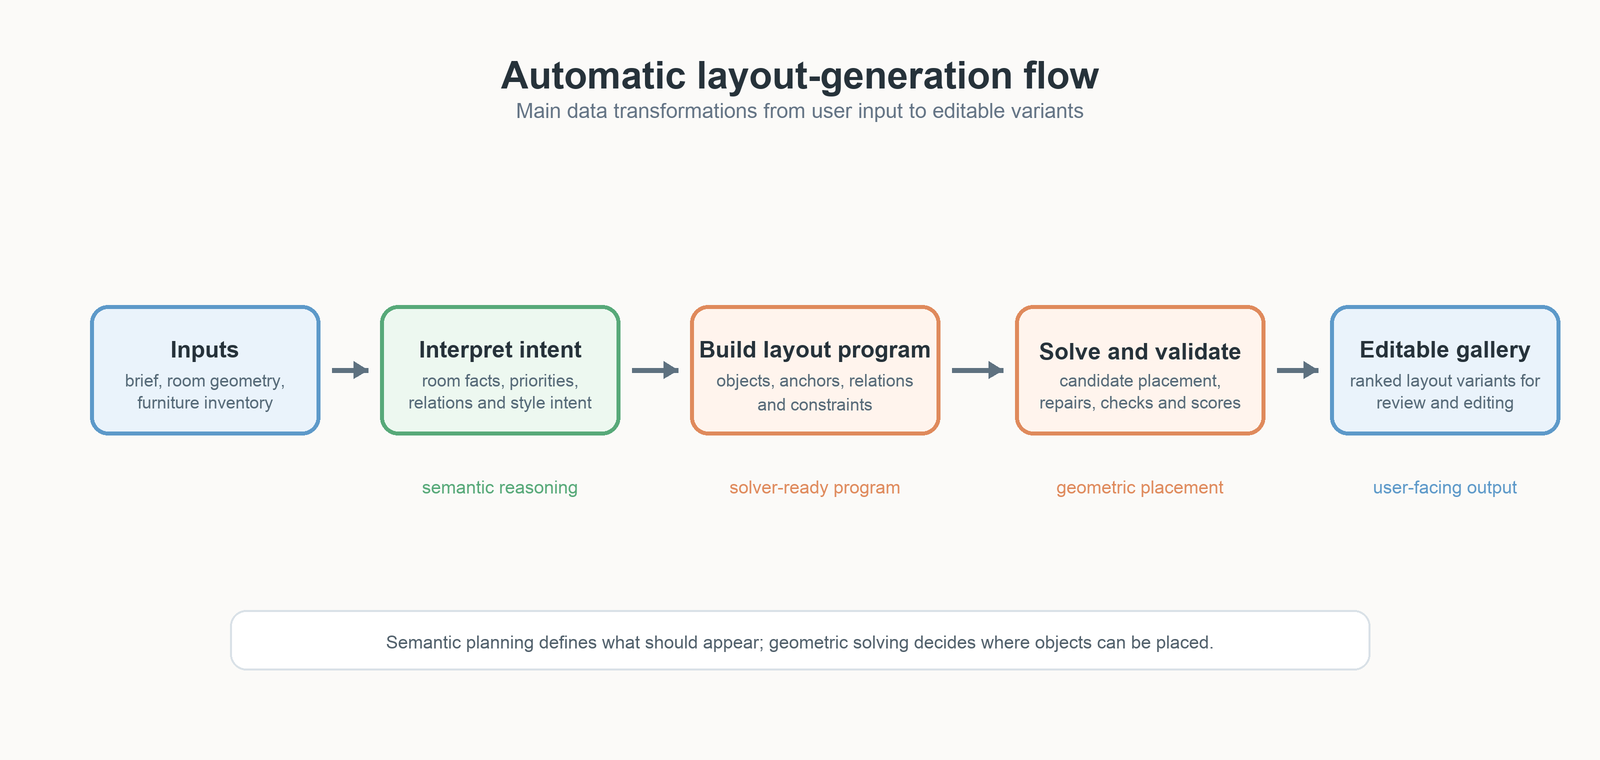
\includegraphics[width=0.96\textwidth]{figures/chapter4/problem1_flow_overview.png}
\caption{High-level flow from the three input sources to an editable layout gallery.}
\label{fig:4-1}
\end{figure}

\hyperref[fig:4-1]{Figure~4.1} first shows the pipeline at the level of its main data transformations. \hyperref[fig:4-2]{Figure~4.2} expands the same pipeline into five module groups. Room interpretation normalizes the design case and fixed room geometry. Semantic planning compiles style preferences, functional clusters, request priorities, and tier/count decisions. The layout-program group merges these decisions into anchor-first concepts and solver relation plans. Geometric solving places the objects, repairs near-valid candidates, and scores feasible layouts. Finalization restores eligible accessories, binds inventory and style metadata, and selects a small gallery of distinct editable variants.

\begin{figure}[!htbp]
\centering
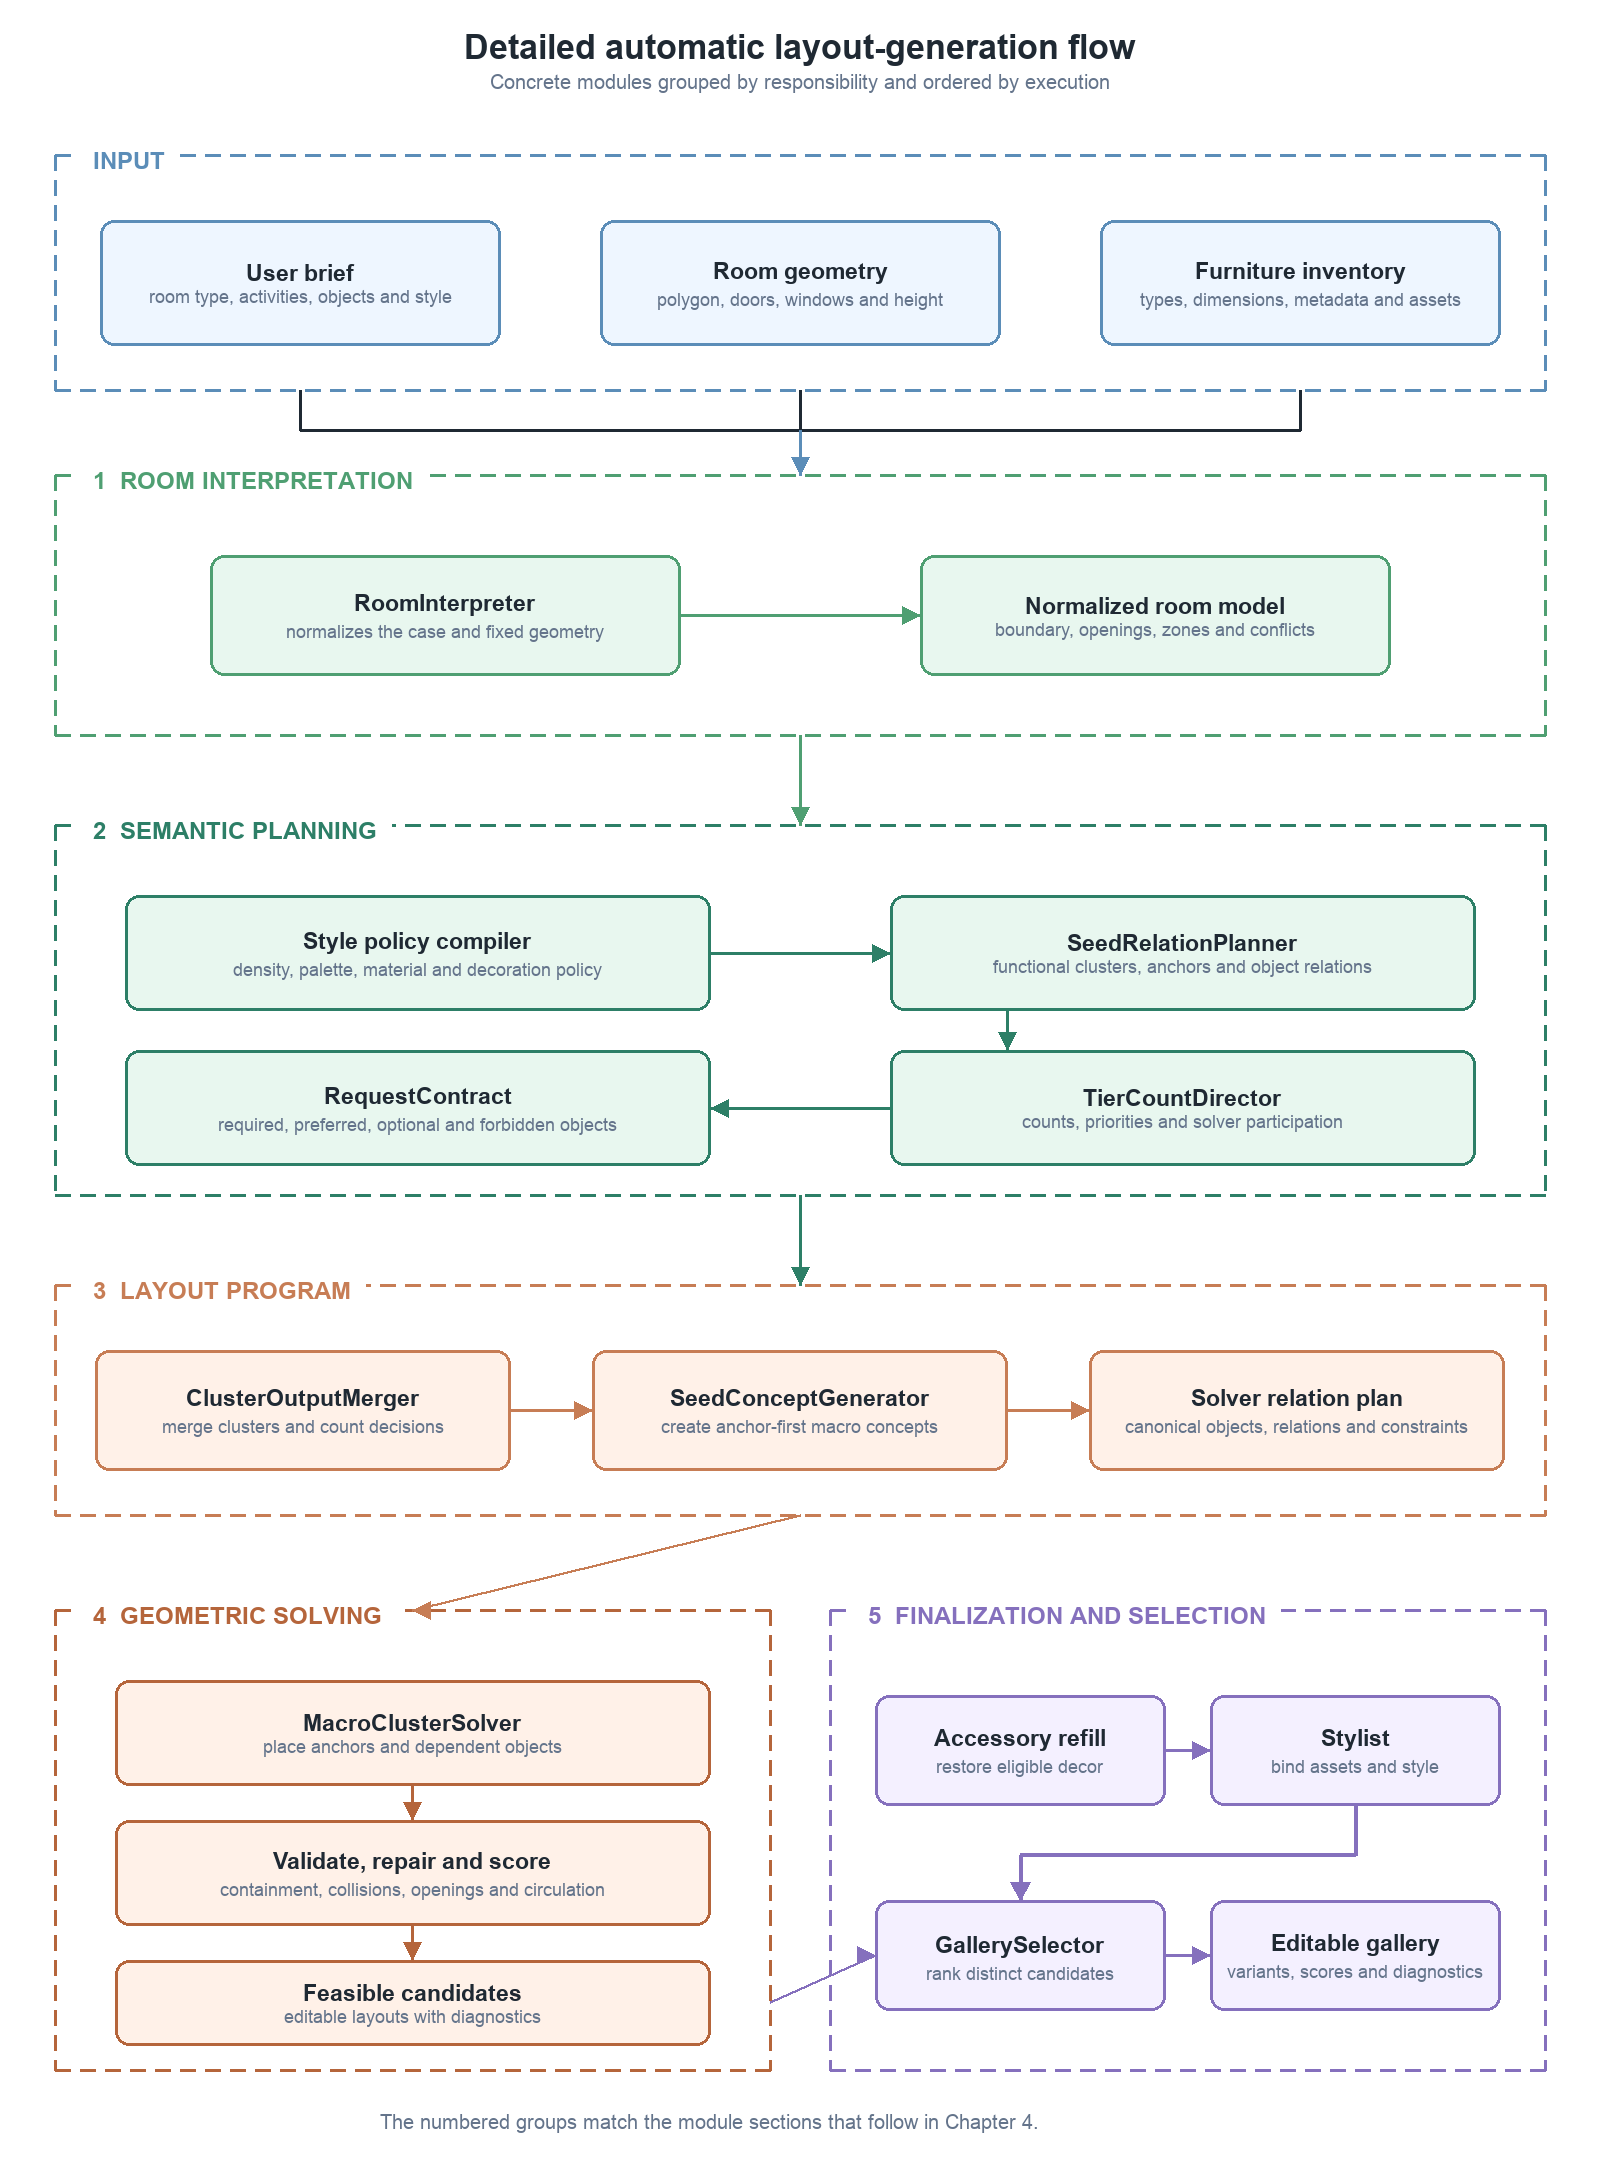
\includegraphics[width=0.98\textwidth]{figures/chapter4/problem1_flow_detailed.png}
\caption{Detailed module groups and intermediate artifacts in automatic layout generation.}
\label{fig:4-2}
\end{figure}

The module names in \hyperref[fig:4-2]{Figure~4.2} refer to processing stages rather than independent system actors. Each stage transforms the case into a more structured form. Early stages extract room facts, style intent, and furniture priorities. Middle stages build object groups, anchors, and solver constraints. Later stages validate concrete placements and select user-facing variants. This interpretation keeps the diagram focused on data flow and prevents the modules from being confused with use case actors.

The final output of the pipeline is not a static image. It is a structured layout gallery in which each variant contains furniture objects, positions, orientations, scores, and diagnostic information. A simplified output format is shown below.

\noindent\begin{minipage}{\linewidth}
\begin{verbatim}
{
  "case_id": "bedroom_compact_001",
  "variants": [
    {
      "variant_id": "v1",
      "score": {"overall": 94.8, "geometry": 100.0},
      "objects": [
        {"id": "bed_1", "type": "bed",
         "center_mm": [1100, 1700], "rotation_deg": 0},
        {"id": "desk_1", "type": "desk",
         "center_mm": [3150, 850], "rotation_deg": 180}
      ],
      "diagnostics": {"violations": []}
    }
  ]
}
\end{verbatim}
\end{minipage}

This separation is important because language models can describe plausible rooms, but they do not by themselves guarantee geometric validity. In RoomFlow, semantic reasoning decides what should appear in the room and why it is needed. The solver then decides where objects can be placed while preserving room boundaries, avoiding overlap, keeping openings usable, and leaving circulation space. This design keeps the layout both controllable for the system and editable for the user.

\section{Input Representation}\label{sec:problem1-input-representation}

Each pipeline run is represented as a structured design case. The case keeps the user's semantic request separate from physical room data and furniture records. This separation allows the language-model modules to interpret intent without inventing geometry, while the later modules work with explicit dimensions and identifiers.

The complete implementation schema contains additional identifiers, metadata, and diagnostic fields used by the backend and benchmark runners. The main text shows only the fields needed to understand the data flow. The design brief records room type, intended activities, required furniture, and style preferences. The room input stores the polygon in millimeters, fixed openings, and room height. The inventory scope identifies the furniture categories available to the pipeline. In the simplified example, each opening is attached to a named wall and its \texttt{span\_mm} is measured along that wall's direction. The implementation also stores wall-edge metadata and the opening position in the room coordinate system, allowing the solver to derive clearance zones and reject furniture that blocks the opening.

\noindent\begin{minipage}{\linewidth}
\begin{verbatim}
{
  "brief": "compact bedroom with a bed, wardrobe and desk",
  "room": {
    "polygon_mm": [[0,0], [4000,0], [4000,3200], [0,3200]],
    "openings": [
      {"id": "door_1", "type": "door",
       "wall": "south", "span_mm": [600,1500]},
      {"id": "window_1", "type": "window",
       "wall": "north", "span_mm": [1800,2800]}
    ]
  },
  "inventory_scope": ["bed", "wardrobe", "desk", "chair"]
}
\end{verbatim}
\end{minipage}

The same identifiers and millimeter coordinate system are retained throughout the pipeline. As a result, semantic requirements, solver decisions, 2D editing, 3D reconstruction, and evaluation artifacts can be traced back to the same design case.

\section{Semantic Planning Module}\label{sec:problem1-semantic-planning-module}

The semantic planning module determines which furniture items are needed and how they should relate to one another. A user rarely provides a complete object list. For example, a request for ``a cozy guest bedroom with storage and a small vanity near the window'' implies a bed, wardrobe, lighting, a vanity desk, and supporting furniture, but the exact priorities and quantities still need to be inferred before placement begins.

The module uses LLM-assisted planning to create structured requirements rather than final coordinates. A style-policy compiler translates terms such as ``minimal'', ``boho'', or ``warm'' into density, palette, material, and decoration preferences. A relation planner groups objects into functional clusters. A request-contract builder classifies objects as required, preferred-if-fit, optional, or forbidden. A count director determines how many instances should participate in the placement problem.

Figure~\ref{fig:4-3} summarizes this semantic-planning flow from the user brief to request contracts, relations, quantities, and style policy.

\begin{figure}[!htbp]
\centering
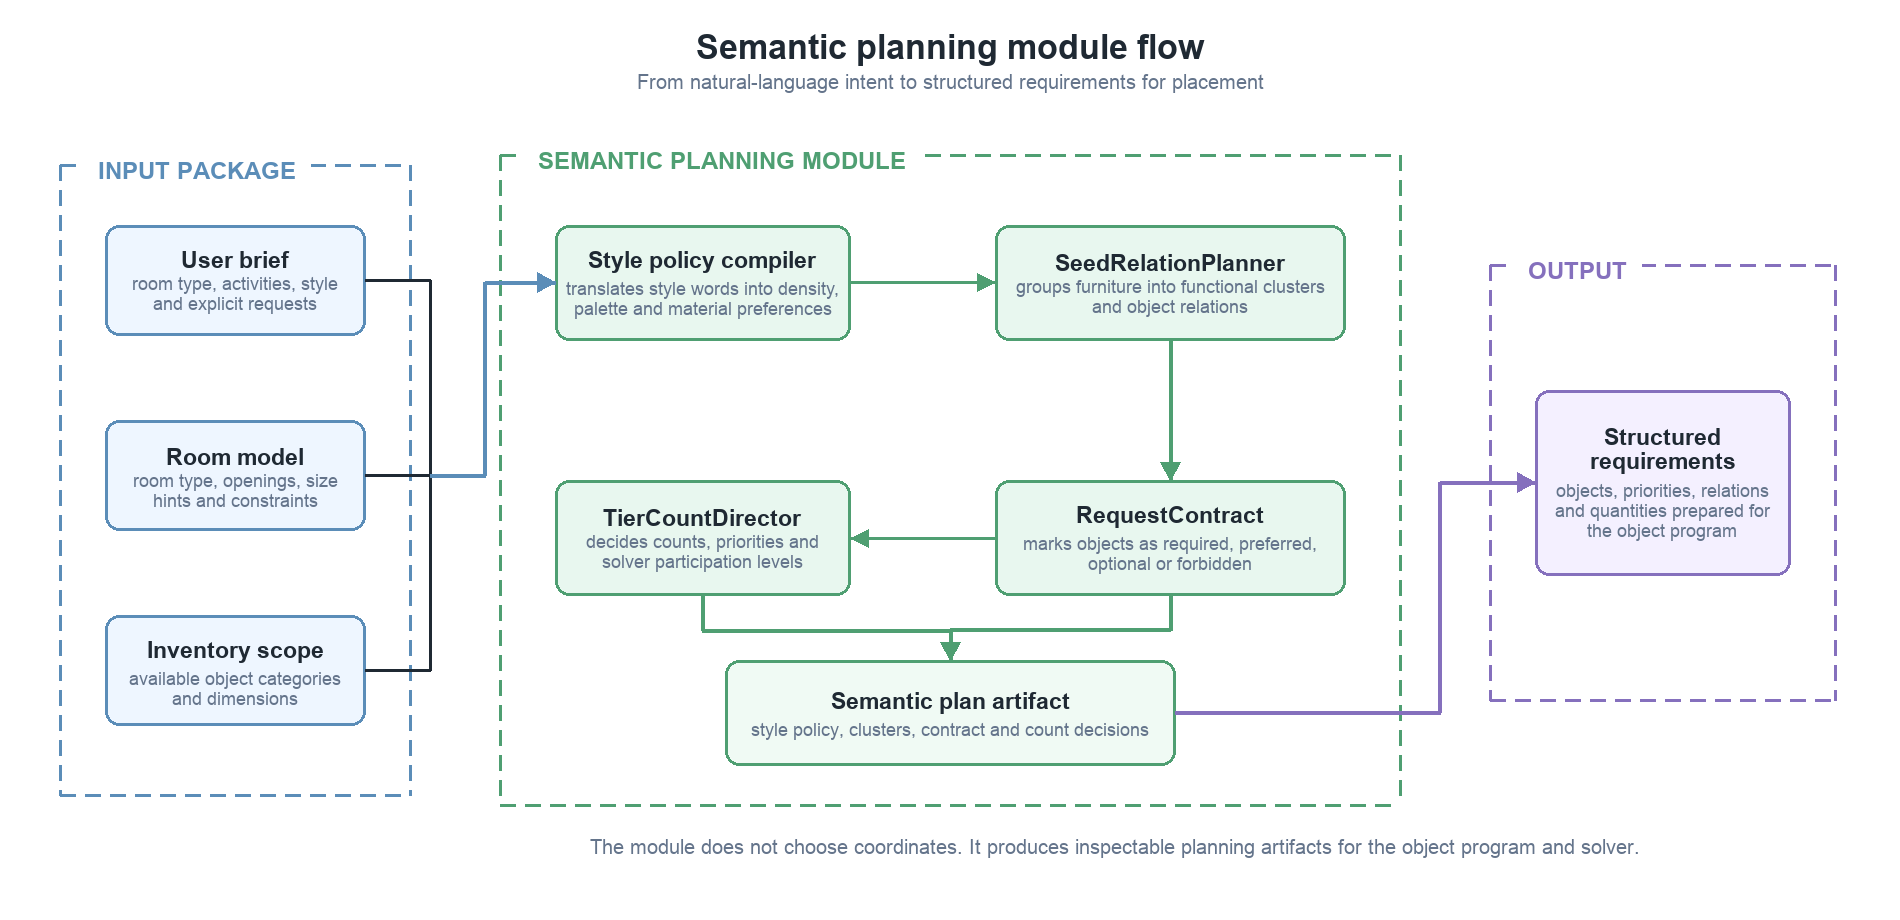
\includegraphics[width=0.98\textwidth]{figures/chapter4/semantic_planning_flow.png}
\caption{Flow of the semantic planning module.}
\label{fig:4-3}
\end{figure}

The following shortened example shows the main input and output of the module.

\noindent\begin{minipage}{\linewidth}
\begin{verbatim}
Input:
{"brief": "cozy guest bedroom with storage",
 "extra_request": "small vanity near the window"}

Output:
{"required": ["bed", "wardrobe"],
 "preferred_if_fit": ["vanity_desk", "chair"],
 "quantities": {"bed": 1, "wardrobe": 1,
                  "vanity_desk": 1, "chair": 1},
 "relations": [["vanity_desk", "near", "window"]],
 "style_policy": {"density": "medium", "materials": ["wood"]}}
\end{verbatim}
\end{minipage}

The request contract protects the user's intent during later pruning. If the room is too small, the solver may omit a decorative object, but it should not silently remove a required bed or wardrobe.

The output of this module is not a final layout. It is a structured semantic plan that records required and optional objects, preferred relations, quantities, and style or material preferences. The object-program module converts this plan into active objects, anchors, relation templates, hard constraints, and soft preferences that the geometric solver can use.

Table~\ref{tab:4-1} lists the main semantic planning stages together with their validation and fallback behavior.

\begingroup
\small
\setlength{\tabcolsep}{4pt}
\renewcommand{\arraystretch}{1.15}
\begin{xltabular}{\textwidth}{|>{\raggedright\arraybackslash}p{3.2cm}|>{\raggedright\arraybackslash}X|>{\raggedright\arraybackslash}X|>{\raggedright\arraybackslash}X|}
\caption{Semantic planning stages, validation rules, and fallback behavior.}\label{tab:4-1}\\
\hline
Stage & Input & Output & Validation and fallback \\
\hline
Style policy & Brief, room type & Density, palette, material, decor preferences & Missing style is mapped to a neutral default; invalid tags are ignored. \\
\hline
Relation planning & Object candidates and activities & Functional clusters and relations & Unsupported relations are dropped or converted to soft preferences. \\
\hline
Request contract & Brief and inferred objects & Required, preferred-if-fit, optional, forbidden objects & Explicit user requests and room-primary objects become required; optional objects are first to prune when infeasible. \\
\hline
Tier/count decision & Contract, inventory, room size & Number of participating objects per category & Counts are clipped by inventory availability and room capacity. \\
\hline
\end{xltabular}
\endgroup

\section{Room Modeling Module}\label{sec:problem1-room-modeling-module}

The room modeling module uses a compact 2D-first room representation, where the room boundary, openings, furniture footprints, height, orientation, and metadata share the same millimeter coordinate system. This representation is inspired by floor-plan-and-object abstractions in indoor scene synthesis \cite{Paschalidou2021AtissAutoregressiveTransformers}, \cite{Tang2024DiffusceneDenoisingDiffusion}, but it is not copied as a fixed formula. RoomFlow simplifies the scene model for interactive editing and adds application-specific opening metadata, clearance zones, wall anchors, circulation targets, and render-facing metadata.

The module's main role is to transform user-drawn geometry into solver-ready constraints. It converts UI coordinates into millimeters, checks that the polygon is valid, attaches each opening to a wall segment, and derives clearance zones, wall-anchor candidates, circulation targets, and daylight hints. This step blocks malformed drawings before they reach the solver. It does not model structural layers, electrical systems, plumbing, or construction documents. It retains only the information required for furniture placement, validation, editing, 3D preview, and image conditioning.

Before solving, the room modeling module normalizes and validates the user-drawn geometry. It first converts UI coordinates into millimeters and orders polygon vertices consistently. It then rejects self-intersecting or too-small polygons because they cannot represent valid rooms. Each door or window is attached to the nearest wall segment only when the distance is within a defined tolerance; otherwise, the user must correct the opening placement. Finally, the module derives clearance polygons, wall-anchor candidates, circulation targets, and daylight hints. These checks make the solver input deterministic and prevent malformed drawings from being treated as valid rooms.

Figure~\ref{fig:4-4} illustrates how the raw room polygon and openings are converted into validated room features and solver constraints.

\begin{figure}[!htbp]
\centering
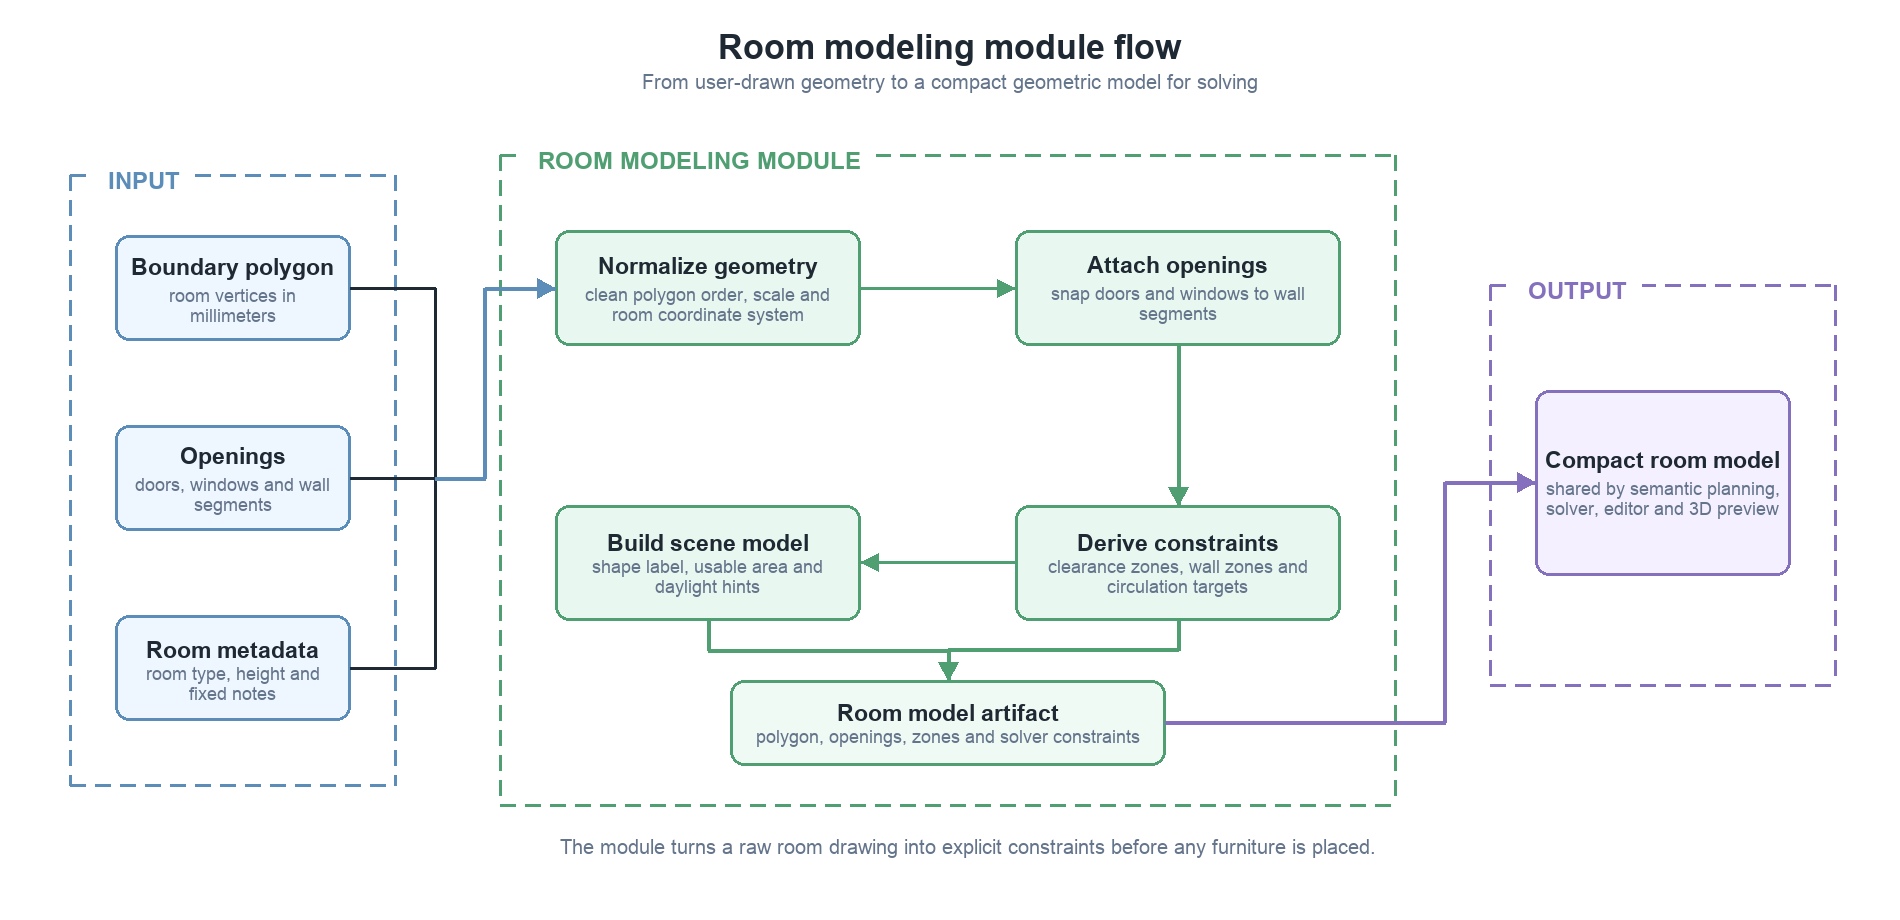
\includegraphics[width=0.98\textwidth]{figures/chapter4/room_modeling_flow.png}
\caption{Flow of the room modeling module.}
\label{fig:4-4}
\end{figure}

\noindent The reduced example below shows only the fields required to understand this transformation.

\noindent\begin{minipage}{\linewidth}
\begin{verbatim}
Input:
{"polygon_mm": "L-shaped polygon",
 "openings": ["door_1", "window_1"]}

Output:
{"shape": "non_rectangular_l_shape",
 "clearance_zones": ["door_1_clearance"],
 "circulation_targets": ["room_center"],
 "daylight_zone": "window_1"}
\end{verbatim}
\end{minipage}

The resulting room model gives later modules more information than a raw polygon. It identifies where openings must remain usable, which walls can anchor large furniture, and which areas should remain open for circulation.

\section{Object Program and Geometric Solver}\label{sec:problem1-object-program-and-solver}

The object program module converts the request contract and room model into a structured placement problem. It identifies active objects, anchor objects, support objects, hard constraints, soft preferences, and accessories that can be added after the main layout is valid. An anchor determines the structure of a functional group, such as a bed in a bedroom or a sofa in a living room. A support object depends on that anchor, such as a nightstand beside a bed or a chair paired with a desk.

Figure~\ref{fig:4-5} shows how this object program is connected to geometric solving, validation, repair, and layout scoring.

\begin{figure}[!htbp]
\centering
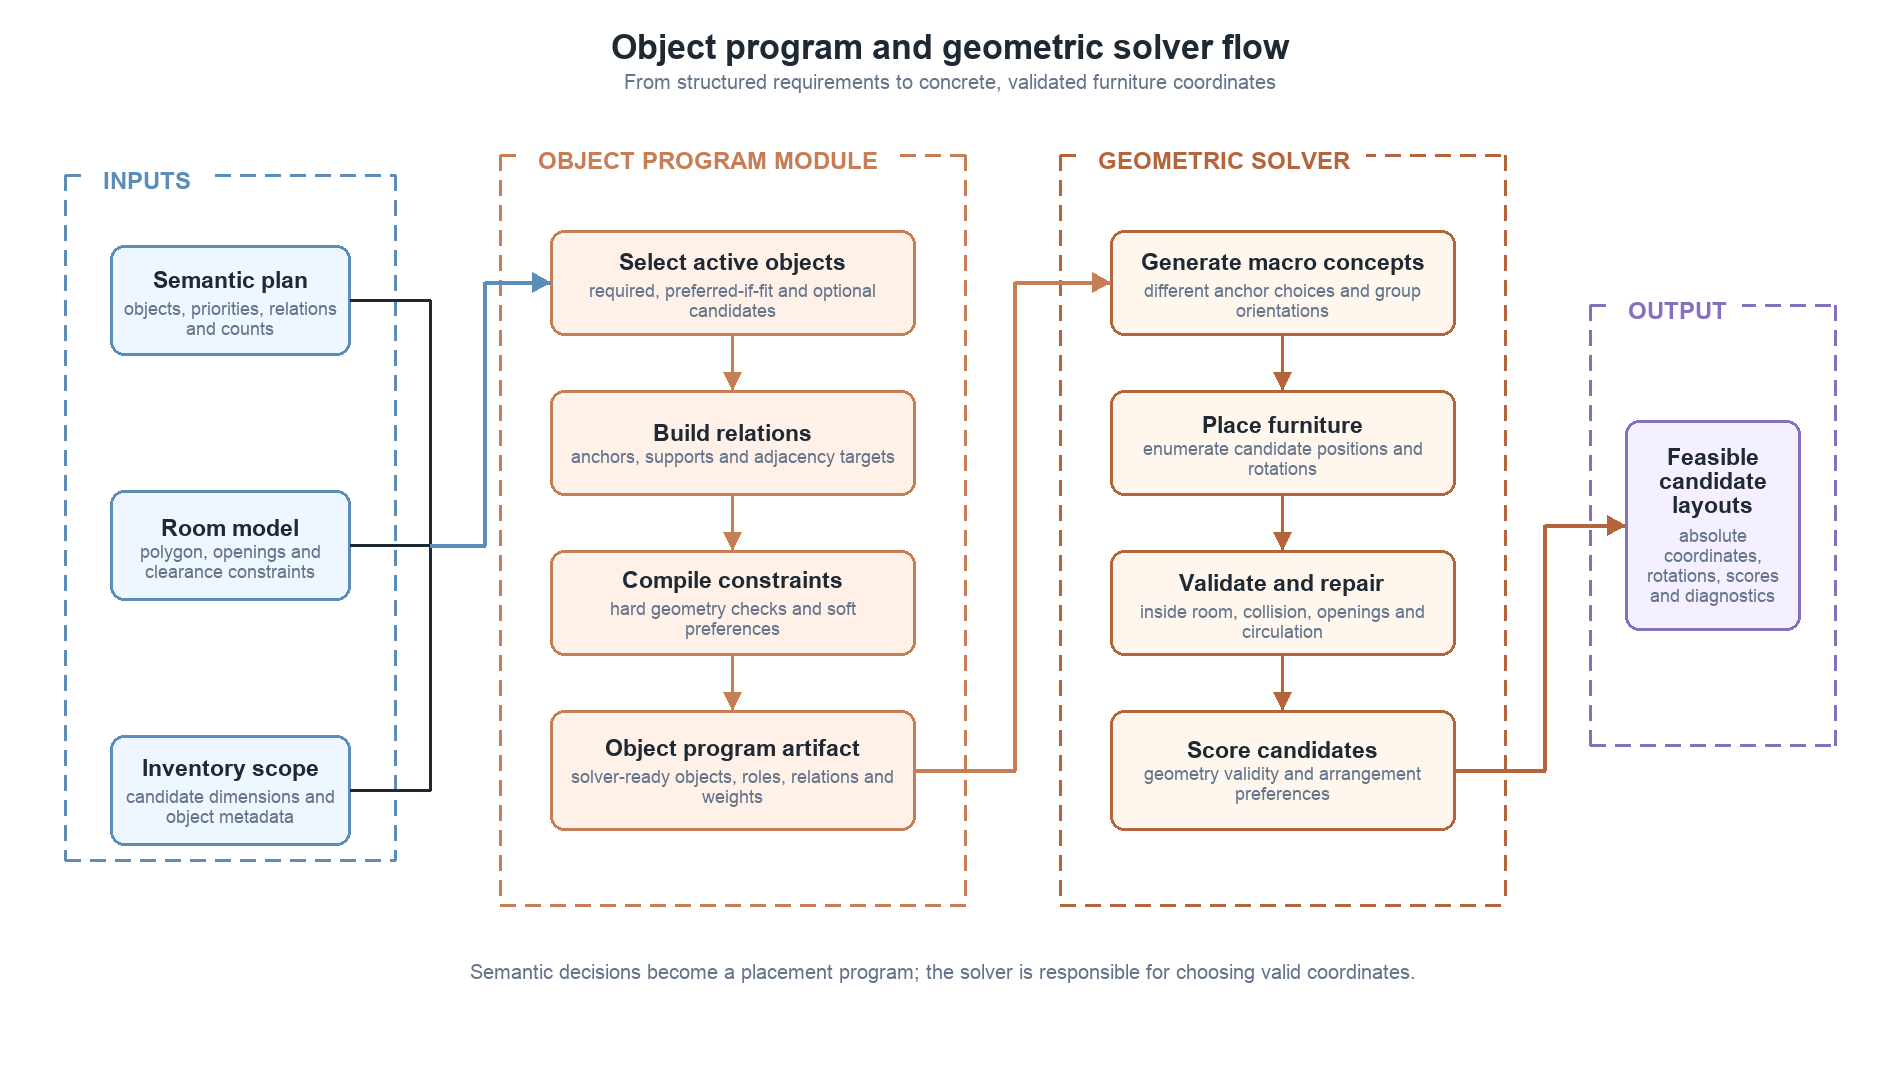
\includegraphics[width=0.98\textwidth]{figures/chapter4/object_program_solver_flow.png}
\caption{Flow from object program construction to geometric solving.}
\label{fig:4-5}
\end{figure}

\noindent\begin{minipage}{\linewidth}
\begin{verbatim}
{
  "objects": [
    {"type": "bed", "role": "anchor", "priority": "required"},
    {"type": "wardrobe", "role": "anchor", "priority": "required"},
    {"type": "nightstand", "role": "support", "anchor": "bed"}
  ],
  "relations": [["nightstand", "beside", "bed"]]
}
\end{verbatim}
\end{minipage}

The geometric solver then enumerates and validates concrete placements. Classical furniture-layout systems encode design guidelines and optimize or sample arrangements according to accessibility, visibility, and spatial relationships \cite{Merrell2011InteractiveFurnitureLayout}, \cite{Yu2011MakeHomeAutomatic}. RoomFlow adapts this constraint-based view to its application workflow through deterministic enumeration, repair, validation, and scoring over the compact room model. The constraint equations below are therefore RoomFlow's implementation notation, not formulas copied unchanged from those references; they keep the relevant containment, collision, opening, and circulation checks and connect them to editable layout diagnostics.

\noindent The geometric solver uses an anchor-first heuristic search rather than a learned model or an exact global optimizer. It enumerates candidate anchor positions and orientations, attaches dependent objects from relation templates, repairs near-valid placements when possible, and ranks feasible layouts with rule-based scores. This design makes failures easier to inspect and fits the thesis goal of producing reliable editable layouts.

The solver procedure can be summarized as Algorithm 1. The algorithm first enumerates anchors for required objects, then attaches dependent objects, repairs near-valid layouts, and finally scores feasible candidates.

\noindent\textbf{Algorithm 1: Anchor-first geometric search for editable layout generation.}

{\footnotesize
\begin{verbatim}
Input: room model, object program, inventory dimensions
Output: ranked candidate layouts

1. Generate wall, corner, center, and relation-based anchor targets.
2. Enumerate orientations for primary anchor objects.
3. Place required anchors; reject hard-constraint violations.
4. Attach support objects from relation templates.
5. Repair near-valid candidates by shifting objects within allowed zones.
6. Add optional accessories only after blocking furniture is valid.
7. Score feasible candidates with soft objectives.
8. Keep ranked candidates and diagnostics for gallery selection.
\end{verbatim}
}

The ranked candidates and diagnostics are used by the gallery selector and the frontend. Valid candidates become selectable layout variants. The associated diagnostics explain unsatisfied requirements, such as a required object that is too large for the room or an opening that cannot remain clear.

The hard constraints reject physically unusable layouts:

\begin{align*}
R_i(\theta_i) &\subseteq P_{\mathrm{room}}, \\
\operatorname{area}(R_i(\theta_i) \cap R_j(\theta_j)) &= 0, \quad i \neq j, \\
\operatorname{dist}(R_i(\theta_i), g_k) &\geq \delta_k, \\
\operatorname{path}(g_k, \operatorname{center}(P_{\mathrm{room}})) &\text{ is unblocked.}
\end{align*}

The soft objective ranks feasible layouts by design preferences:

\[
L^{\star} = \arg\min_{L \in \mathcal{F}} E(L), \quad
E(L) = \sum_m \lambda_m \phi_m(L) + \sum_n \mu_n \psi_n(L)
\]

Candidates that violate hard constraints are rejected before this ranking step. In the remaining feasible set, the \(\phi_m\) terms record residual geometric risk or repair cost, while the \(\psi_n\) terms express preferences such as wall anchoring, visibility, adjacency, balance, and circulation. The solver uses an anchor-first strategy: it places the main object of each functional cluster before dependent furniture and decoration.

Table~\ref{tab:4-2} summarizes the hard and soft objective terms used to rank feasible layout candidates.

\begingroup
\small
\setlength{\tabcolsep}{4pt}
\renewcommand{\arraystretch}{1.15}
\begin{xltabular}{\textwidth}{|>{\raggedright\arraybackslash}p{2.8cm}|>{\raggedright\arraybackslash}X|>{\raggedright\arraybackslash}X|>{\raggedright\arraybackslash}p{1.8cm}|}
\caption{Main solver objective terms used in layout ranking.}\label{tab:4-2}\\
\hline
Term & Purpose & Scoring rule & Weight role \\
\hline
Containment and overlap & Reject physically invalid layouts & Reject if blocking footprints leave the room or intersect & Hard \\
\hline
Opening clearance & Keep doors and windows usable & Reject if a door/window clearance zone or entry path is blocked & Hard \\
\hline
Wall anchoring & Prefer large objects near suitable walls & Reward small distance to candidate wall anchors when appropriate & Soft \\
\hline
Functional adjacency & Keep related objects usable together & Reward relation templates such as nightstand beside bed or sofa facing media unit & Soft \\
\hline
Visibility and circulation & Preserve view lines and walking space & Reward open center regions and penalize path blockers & Soft \\
\hline
Balance & Avoid all objects collapsing into one corner & Penalize extreme distribution imbalance when it hurts use & Soft \\
\hline
\end{xltabular}
\endgroup

A validated candidate stores concrete placements together with hard-check and score summaries:

\noindent\begin{minipage}{\linewidth}
\begin{verbatim}
{
  "layout_id": "candidate_07",
  "objects": [
    {"id": "bed_1", "center_mm": [1250,1900], "rotation_deg": 0}
  ],
  "hard_checks": {"inside_room": true, "openings_clear": true},
  "score": {"overall": 94.8}
}
\end{verbatim}
\end{minipage}

\section{Gallery Selection and Editable Output}\label{sec:problem1-gallery-selection}

The gallery selector converts many feasible solver candidates into a small set of user-facing variants. It first rejects candidates below the hard-validity threshold. Near-valid candidates are kept only when repair removes the violations. The remaining candidates are sorted by score and filtered by a layout signature. The signature records high-level structural choices such as the wall used by the bed or sofa, the orientation of major objects, and the main circulation pattern. For example, two bedroom candidates that both anchor the bed to the north wall, keep the wardrobe on the east wall, and use the same entry path are treated as duplicates even if their coordinates differ slightly. This filtering prevents the gallery from showing many near-identical layouts. After filtering, the selector attaches inventory, material, style, and diagnostic metadata so that the user can compare a few genuinely different options.

Figure~\ref{fig:4-6} shows this finalization step from validated candidates to a compact editable gallery.

\begin{figure}[!htbp]
\centering
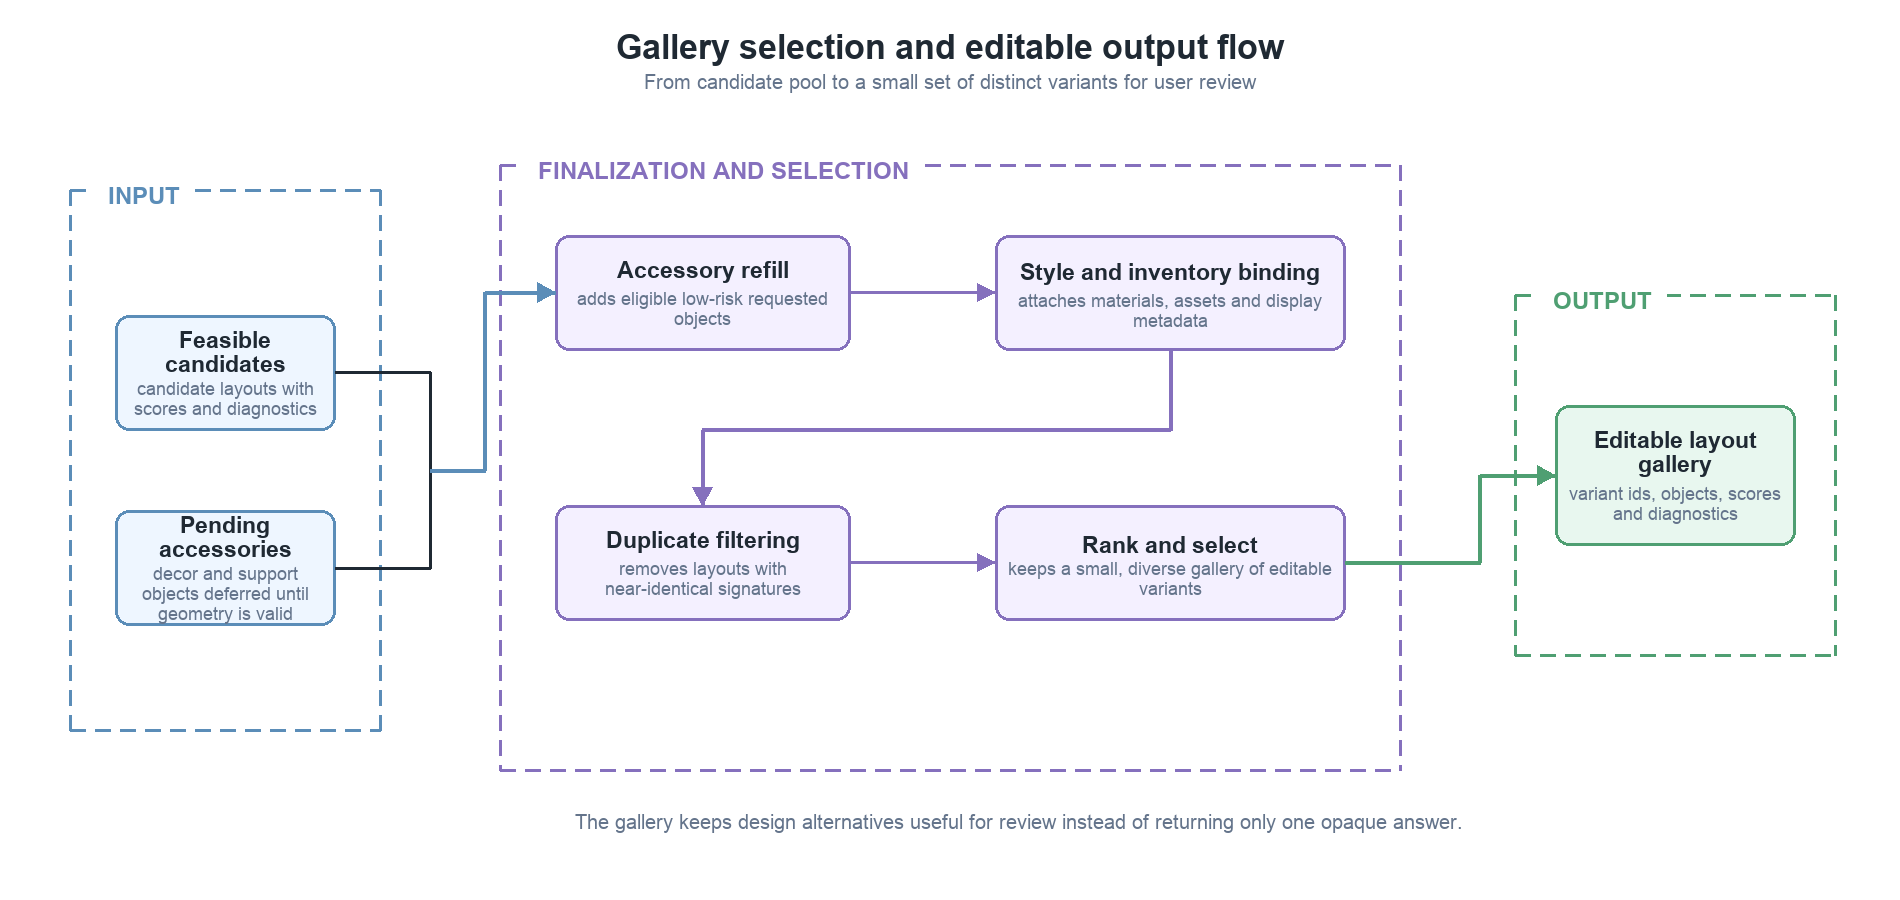
\includegraphics[width=0.98\textwidth]{figures/chapter4/gallery_selection_flow.png}
\caption{Flow of gallery selection and editable output preparation.}
\label{fig:4-6}
\end{figure}

The selected variant and its alternatives are returned as editable application state rather than rendered pixels:

\noindent\begin{minipage}{\linewidth}
\begin{verbatim}
{
  "selected_variant_id": "candidate_07",
  "alternatives": ["candidate_03", "candidate_11"],
  "editable_state": {"object_count": 12, "violations": 0}
}
\end{verbatim}
\end{minipage}

Every placed object retains its id, type, dimensions, center point, rotation, height, front direction, and metadata. The 2D editor uses this state for direct manipulation, the 3D preview reconstructs the room from it, and the image-generation workflow uses it to prepare a layout-conditioned snapshot. The result directly supports the first thesis objective: users can begin with an automatic layout and continue editing it instead of receiving a static image.

If the gallery is empty, the system returns diagnostics instead of a silent failure. Typical diagnostics include required object too large for the room, opening clearance blocked by all attempted placements, or no valid relation template for the requested furniture combination. These diagnostics allow the user to relax optional requirements, change the room input, or continue with manual editing.
